\section{auswertung}

\subsection{Nulleffekt}
Die gemessen Impulse ohne Präparat in einem Intervall von $\Delta t = 300\si{s}$ ergben.
\begin{equation*}
N_U= \{ 129, 143, 144, 136, 139, 126, 158 \}
\end{equation*}
Die Fehler der gemessenen Werte des Nulleffekts werden jeweils durch eine Poisson Verteilung herausgefunden.
Da es eine Vielzahl an Messungen gibt, werden die resultierenden Fehler anschließend gemittelt.
Nach der Poisson Verteilung sieht der Fehler auf $N$ aus wie folgt
\begin{align}
\label{eqn:mittel}
\Delta N &= \sqrt{N}
\intertext{Diesen gilt es wiederum über die Anzahl der Messungen zu mitteln}
 \bar{\Delta N} &= \frac{1}{n} \sum_{i=1}^n \Delta N_i% BAR MUSS GRÖ?ER
\intertext{mit ensprechende werten (siehe Anhang) ergibt sich als Mitteltwert der Poission Verteilung und somit als finalen Wert des Nulleffekts} % idk obd as schön ist, bzw ob das geht
\bar{\Delta N} & = \si{139}{\pm4}
\end{align}
Das Mittel des Nulleffekts auf einem Intervall von $\Delta t = 300\si{s}$ ist nun also bekannt. Um den Effekt auf die kommenden Aufgaben anzupassen 
wird $\bar{\Delta N}$ mit einem Dreisatz, den Fehler natürlich miteinbeziehend, angepasst. 
\begin{align}
\bar{\Delta N_{30}} &= 13.9\pm 0.4 [\frac{Imp}{30\si{s}}] \\                %schöner machen
\bar{\Delta N_{15}} &= 6.96\pm 0.22 [\frac{Imp}{30\si{s}}]
\end{align}
\\
\paragraph{mittelung der messwerte von Vanadium} \mbox{} \\
Analog zu \eqref{eqn:mittel} lässt sich durch die Poisson Verteilung der Fehler auf  die Werte bestimmnen. Die genauen Ergbnisse befinden sich im Anhang.


\begin{figure}
  \centering
  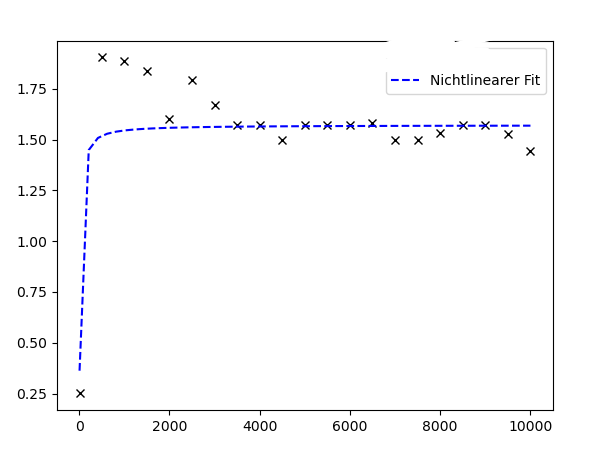
\includegraphics[width=0.8\textwidth]{build/plot1.pdf}
  \caption{$t-N$ Diagramm.}
  \label{fig:tndiagramm}
\end{figure}


